\section{Ejercicio 4 - Conversor a codigo de Gray}
Para esté ejercicio, realizamos el desarrollo de un circuito lógico capaz de convertir un número binario de 4 bits a su equivalente de código de Gray, esto resulta en la siguiente tabla de verdad:
\begin{table}[H]
	\begin{center}
		\begin{tabular}{|c|c|c|c||c|c|c|c|}
			\hline
			\multicolumn{4}{|c||}{Entrada} & \multicolumn{4}{|c|}{Salida}\\
			\hline
			$X_1$ &	$X_2$ &	$X_3$ &	$X_4$ & $Y_1$ & $Y_2$ & $Y_3$ & $Y_4$\\
			\hline
			0 & 0 & 0 & 0 & 0 & 0 & 0 & 0\\
			\hline
			0 & 0 & 0 & 1 & 0 & 0 & 0 & 1\\
			\hline
			0 & 0 & 1 & 0 & 0 & 0 & 1 & 1\\
			\hline
			0 & 0 & 1 & 1 & 0 & 0 & 1 & 0\\
			\hline
			0 & 1 & 0 & 0 & 0 & 1 & 1 & 0\\
			\hline
			0 & 1 & 0 & 1 & 0 & 1 & 1 & 1\\
			\hline
			0 & 1 & 1 & 0 & 0 & 1 & 0 & 1\\
			\hline
			0 & 1 & 1 & 1 & 0 & 1 & 0 & 0\\
			\hline
			1 & 0 & 0 & 0 & 1 & 1 & 0 & 0\\
			\hline
			1 & 0 & 0 & 1 & 1 & 1 & 0 & 1\\
			\hline
			1 & 0 & 1 & 0 & 1 & 1 & 1 & 1\\
			\hline
			1 & 0 & 1 & 1 & 1 & 1 & 1 & 0\\
			\hline
			1 & 1 & 0 & 0 & 1 & 0 & 1 & 0\\
			\hline
			1 & 1 & 0 & 1 & 1 & 0 & 1 & 1\\
			\hline
			1 & 1 & 1 & 0 & 1 & 0 & 0 & 1\\
			\hline
			1 & 1 & 1 & 1 & 1 & 0 & 0 & 0\\
			\hline
		\end{tabular}
	\end{center}
\end{table}
De la tabla de verdad obtenemos las siguientes ecuaciones en función de los mintérminos:
\begin{center}
	$Y_4=m_1+m_2+m_5+m_6+m_9+m_{10}+m_{13}+m_{14}$\\
	$Y_3=m_2+m_3+m_4+m_5+m_{10}+m_{11}+m_{12}+m_{13}$\\
	$Y_2=m_4+m_5+m_6+m_7+m_8+m_9+m_{10}+m_{11}$\\
	$Y_1=m_8+m_9+m_{10}+m_{11}+m_{12}+m_{13}+m_{14}+m_{15}$\\
\end{center}
Que al reemplazar cada mintérmino por su correspondiente expresión obtenemos:
\begin{center}
	$Y_4=\overline{X_1} \cdot \overline{X_2} \cdot \overline{X_3} \cdot X_4 + 
	\overline{X_1} \cdot \overline{X_2} \cdot X_3 \cdot \overline{X_4} + 
	\overline{X_1} \cdot X_2 \cdot \overline{X_3} \cdot X_4 + 
	\overline{X_1} \cdot X_2 \cdot X_3 \cdot \overline{X_4} + 
	X_1 \cdot \overline{X_2} \cdot \overline{X_3} \cdot X_4 +
	X_1 \cdot \overline{X_2} \cdot X_3 \cdot \overline{X_4} + 
	X_1 \cdot X_2 \cdot \overline{X_3} \cdot X_4 + 
	X_1 \cdot X_2 \cdot X_3 \cdot \overline{X_4}$\\
	\smallskip
	%Empieza la parte Y3%
	$Y_3=\overline{X_1} \cdot \overline{X_2} \cdot X_3 \cdot \overline{X_4} +
	\overline{X_1} \cdot \overline{X_2} \cdot X_3 \cdot X_4 +
	\overline{X_1} \cdot X_2 \cdot \overline{X_3} \cdot \overline{X_4} + 
	\overline{X_1} \cdot X_2 \cdot \overline{X_3} \cdot X_4 + 
	X_1 \cdot \overline{X_2} \cdot X_3 \cdot \overline{X_4} +
	X_1 \cdot \overline{X_2} \cdot X_3 \cdot X_4 + 
	X_1 \cdot X_2 \cdot \overline{X_3} \cdot \overline{X_4} + 
	X_1 \cdot \overline{X_2} \cdot X_3 \cdot X_4$\\
	\smallskip
	%Empieza la parte Y2%
	$Y_2=\overline{X_1} \cdot X_2 \cdot \overline{X_3} \cdot \overline{X_4} + 
	\overline{X_1} \cdot X_2 \cdot \overline{X_3} \cdot X_4 +
	\overline{X_1} \cdot X_2 \cdot X_3 \cdot \overline{X_4} +
	\overline{X_1} \cdot X_2 \cdot X_3 \cdot X_4 +
	X_1 \cdot \overline{X_2} \cdot \overline{X_3} \cdot \overline{X_4} +
	X_1 \cdot \overline{X_2} \cdot \overline{X_3} \cdot X_4 + 
	X_1 \cdot \overline{X_2} \cdot X_3 \cdot \overline{X_4} + 
	X_1 \cdot \overline{X_2} \cdot X_3 \cdot X_4$\\
	\smallskip
	%Empieza la parte Y1%
	$Y_1=X_1 \cdot \overline{X_2} \cdot \overline{X_3} \cdot \overline{X_4} +
	X_1 \cdot \overline{X_2} \cdot \overline{X_3} \cdot X_4 + 
	X_1 \cdot \overline{X_2} \cdot X_3 \cdot \overline{X_4} + 
	X_1 \cdot \overline{X_2} \cdot X_3 \cdot X_4 +
	X_1 \cdot X_2 \cdot \overline{X_3} \cdot \overline{X_4} +
	X_1 \cdot X_2 \cdot \overline{X_3} \cdot X_4 +
	X_1 \cdot X_2 \cdot X_3 \cdot \overline{X_4} +
	X_1 \cdot X_2 \cdot X_3 \cdot X_4$\\
\end{center}
Tenemos unas funciones muy larga y como las tenemos expresadas en mintérminos podemos simplificarlas por medio del mapa de Karnaugh. Ésto nos da a lugar a los siguientes mapas de Karnaugh y funciones de salida simplificadas:\\
\begin{center}
	
\begin{figure}[H]
   \centering
\begin{tabular}{cc}
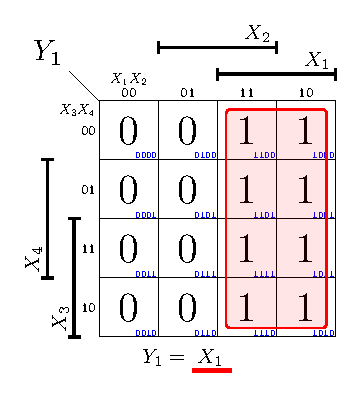
\includegraphics[width=4cm,trim={0.5cm 0.5cm  0.25cm 0.25cm},clip]{Ejercicio_4/Karnaugh/Y_1.pdf}&
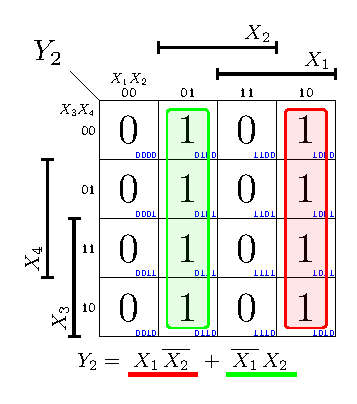
\includegraphics[width=4cm,trim={0.5cm 0.5cm  0.25cm 0.25cm},clip]{Ejercicio_4/Karnaugh/Y_2.pdf}\\
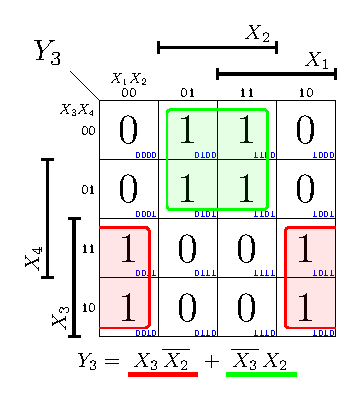
\includegraphics[width=4cm,trim={0.5cm 0.5cm  0.25cm 0.25cm},clip]{Ejercicio_4/Karnaugh/Y_3.pdf}&
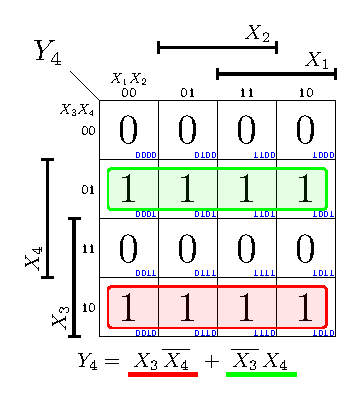
\includegraphics[width=4cm,trim={0.5cm 0.5cm  0.25cm 0.25cm},clip]{Ejercicio_4/Karnaugh/Y_4.pdf}
\end{tabular}
    \caption{Mapas de Karnaugh de las salidas $Y_1$, $Y_2$, $Y_3$ e $Y_4$}
    \label{fig:Karnaughs_GRAY} 
\end{figure}	
   	%Y4
   	$Y_4=X_3 \cdot \overline{X_4}+\overline{X_3} \cdot X_4$
   	\hspace{6mm}
   	%Y3
   	$Y_3=X_2 \cdot \overline{X_3}+\overline{X_2} \cdot X_3$\\
   	%Y4
   	Formula de $Y_4$
   	\hspace{6mm}
   	%Y3
   	Formula de $Y_3$\\
	%Y2
    $Y_2=X_1 \cdot \overline{X_2}+\overline{X_1} \cdot X_2$
    \hspace{6mm}
    %Y1
    $Y_1=X_1$\\
    Formula de $Y_2$
    \hspace{6mm}
    %Y1
    Formula de $Y_1$\\
\end{center}
De los valores obtenidos podemos realizar el siguiente circuito conformado por compuertas OR, AND y NOT:\\
\begin{figure}[H]
	\centering
    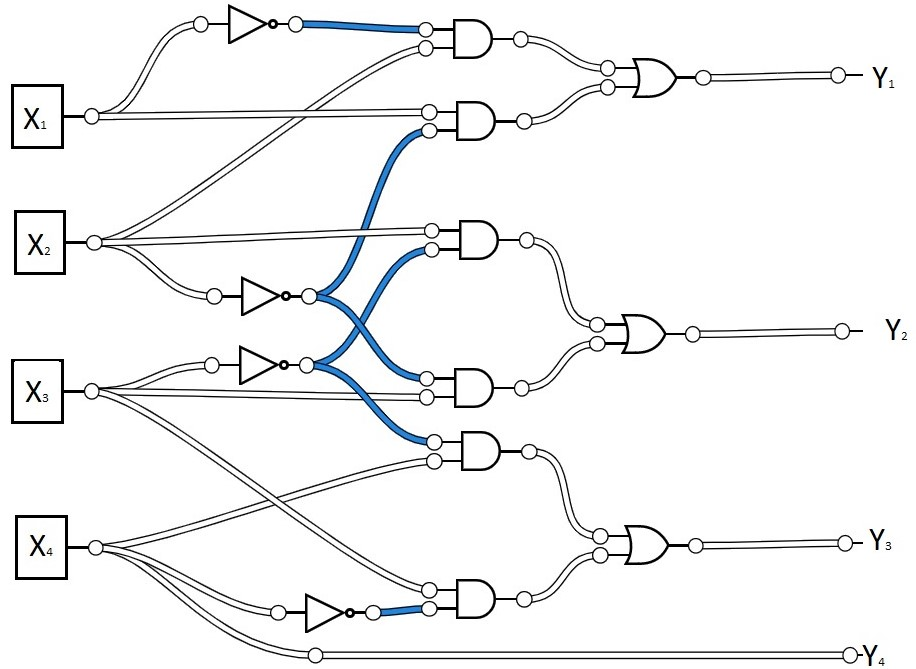
\includegraphics[width=0.5\textwidth]{Ejercicio_4/Circuito}
    \caption{Implementación del conversor a código de Gray}
\end{figure}
